While we have developed equations to model the influence of both SAWs and gravity on the 
motion of thin films, we are primarily concerned with the case where the SAW is the primary driving
force. Hence, for all the simulations shown in this section we use $\beta = 0$. We also use the 
physical characteristics shown in \cref{tab:params}, a precursor film height of $b = 0.01$, as well as a drop initial condition for all the simulations. 
 
\begin{table}[hb]
    \centering
    \begin{tabular}{|lll|}
        \hline
        \multicolumn{3}{|c|}{Parameter Values}                                                                                    \\ \hline
        \multicolumn{1}{|l|}{Symbol}             & \multicolumn{1}{l|}{Physical Meaning}                & Quantitative Value          \\ \hline
        \multicolumn{1}{|l|}{$\rho$}             & \multicolumn{1}{l|}{Density of Oil}                  & 900 $\lrb{\frac{Kg}{m^3}}$  \\
        \multicolumn{1}{|l|}{$g$}                & \multicolumn{1}{l|}{Gravity}                         & 9.8 $\lrb{\frac{m}{s^2}}$   \\
        \multicolumn{1}{|l|}{$\mu$}              & \multicolumn{1}{l|}{Dynamic Viscosity of Oil}        & 0.45 $\lrb{\frac{Kg}{ms}}$                \\
        \multicolumn{1}{|l|}{$\gamma$}           & \multicolumn{1}{l|}{Surface Tension}                 & $20 \times 10^{-3} \lrb{\frac{Kg}{s^2}}$  \\
        \multicolumn{1}{|l|}{$A$}                & \multicolumn{1}{l|}{Amplitude of SAW}                & $8 \times 10^{-10} \lrb{m}$ \\
        \multicolumn{1}{|l|}{$\omega$}           & \multicolumn{1}{l|}{Angular Frequency of SAW}        & $2\pi \times 20 \times 10^6 \lrb{s^{-1}}$ \\
        \multicolumn{1}{|l|}{$\alpha_1$}         & \multicolumn{1}{l|}{Geometric Constant}              & 2.386                       \\
        \multicolumn{1}{|l|}{$k_i^{\text{oil}}$} & \multicolumn{1}{l|}{Attenuation Coefficient in Oil}  & $-1000 \lrb{m^{-1}}$                      \\
        \multicolumn{1}{|l|}{$k_i^{\text{air}}$} & \multicolumn{1}{l|}{Attenuation Coefficient in Air}  & $-1 \lrb{m^{-1}}$                         \\
        \multicolumn{1}{|l|}{$\lambda$}          & \multicolumn{1}{l|}{Steepness of Attenuation Coefficient Change}  & $2 \times 10^{-3} \lrb{m}$                         \\
        \multicolumn{1}{|l|}{$h_c$}              & \multicolumn{1}{l|}{Characteristic Film Thickness}   & $200 \times 10^{−6} \lrb{m}$              \\
        \multicolumn{1}{|l|}{$x_c$}              & \multicolumn{1}{l|}{Characteristic Length Scale}     & $10^{−3} \lrb{m}$           \\
        \multicolumn{1}{|l|}{$t_c$}              & \multicolumn{1}{l|}{Characteristic Time Scale}       & $ .84375 \lrb{s}$           \\
        \multicolumn{1}{|l|}{$\varepsilon$}      & \multicolumn{1}{l|}{Small Parameter}                 & $0.2$                       \\
        \multicolumn{1}{|l|}{$\mathrm{Bo}$}      & \multicolumn{1}{l|}{Bond Number}                     & $0.441$                     \\
        \multicolumn{1}{|l|}{$\mathrm{We_{ac}}$} & \multicolumn{1}{l|}{Acoustic Weber Number}           & $0.45479$                   \\ \hline
    \end{tabular}
    \caption{Physical parameters and their values used in our simulations}
    \label{tab:params}
\end{table}

\subsection{Flat Topography}
In this simulation we consider the scenario where we have a flat topography (i.e. $\func{s}{x} = 0$). This 
corresponds to a single initial drop being moved by SAW forcing with no other liquids in its path. We see in 
\cref{fig:flat_profile} that the initial oil drop moves from left to right and spreads out as it does so, which 
is consistent with experimental observations. We also note the formation of a capillary ridge near the contact line between the oil 
and the surface, which is also consistent with experimental observations. 

\begin{figure}[ht]
    \centering
    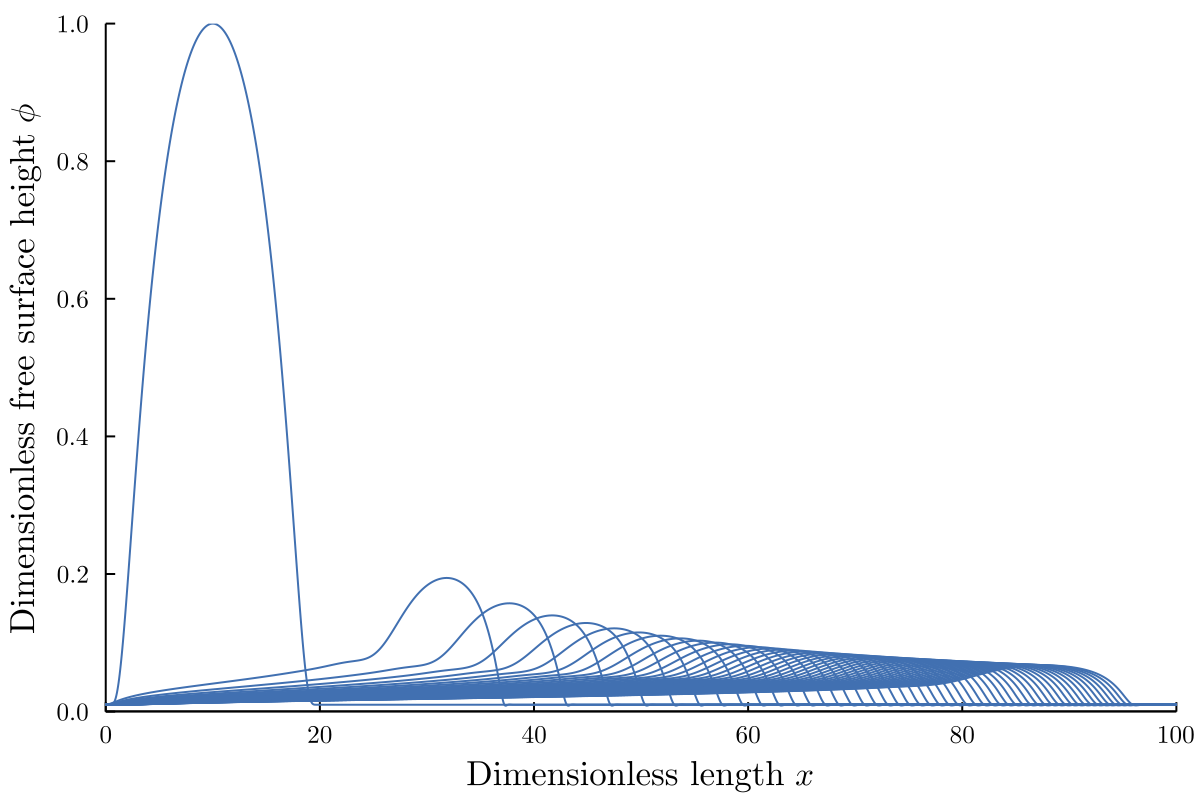
\includegraphics[scale=0.3]{images/flat/plt_notitle.png}
    \caption{Fluid profile on a flat topography plotted every $\Delta t = 10000$ dimensionless time units}
    \label{fig:flat_profile}
\end{figure}

\subsection{Bump Topography}
In the following simulations we consider the scenario where we have a bump topography (see \cref{sec:topography} in the appendix for 
a general bump equation). This corresponds to a single initial drop being moved by SAW forcing with 
another liquid in its path being modelled by the stationary bump.  
In the case where the maximum height of our bump is small, we find that the initial oil drop is able to 
clear the bump and spread over the entire domain as shown in \cref{fig:bump05_profile}. 
However, in the case where the maximum height is large, we find that the initial oil drop is not able to 
clear the bump and gets stuck on it as shown in \cref{fig:bump10_profile}. 
This behavior showcases an inherent limitation of our model in that modelling another liquid as a 
stationary feature of the surface topography does not allow the \textquote{leaky} effects of the surface acoustic wave
to be transferred to the moving liquid as it flows over the bump. Essentially, the effect of acoustic driving 
is lost over the bump region as we consider it to be solid instead of liquid, which is not in acceptance with experimental observations. 
